\documentclass{article}%
\usepackage[T1]{fontenc}%
\usepackage[utf8]{inputenc}%
\usepackage{lmodern}%
\usepackage{textcomp}%
\usepackage{lastpage}%
\usepackage[head=40pt,margin=0.5in,bottom=0.6in]{geometry}%
\usepackage{graphicx}%
%
\title{\textbf{Jubilados del Seniat protestaron en Plaza Venezuela por bajos ingresos}}%
\author{El Nacional Web}%
\date{05/12/2018}%
%
\begin{document}%
\normalsize%
\maketitle%
\textbf{URL: }%
http://www.el{-}nacional.com/noticias/protestas/jubilados{-}del{-}seniat{-}protestaron{-}plaza{-}venezuela{-}por{-}bajos{-}ingresos\_262205\newline%
%
\textbf{Periodico: }%
EN, %
ID: %
262205, %
Seccion: %
Protestas\newline%
%
\textbf{Palabras Claves: }%
Protestas, Gobierno\newline%
%
\textbf{Derecho: }%
2.6, %
Otros Derechos: %
, %
Sub Derechos: %
2.6.1\newline%
%
\textbf{EP: }%
SI\newline%
\newline%
%
\textbf{\textit{Los manifestantes aseguraron que el dinero no les alcanza para cubrir sus necesidades básicas}}%
\newline%
\newline%
%
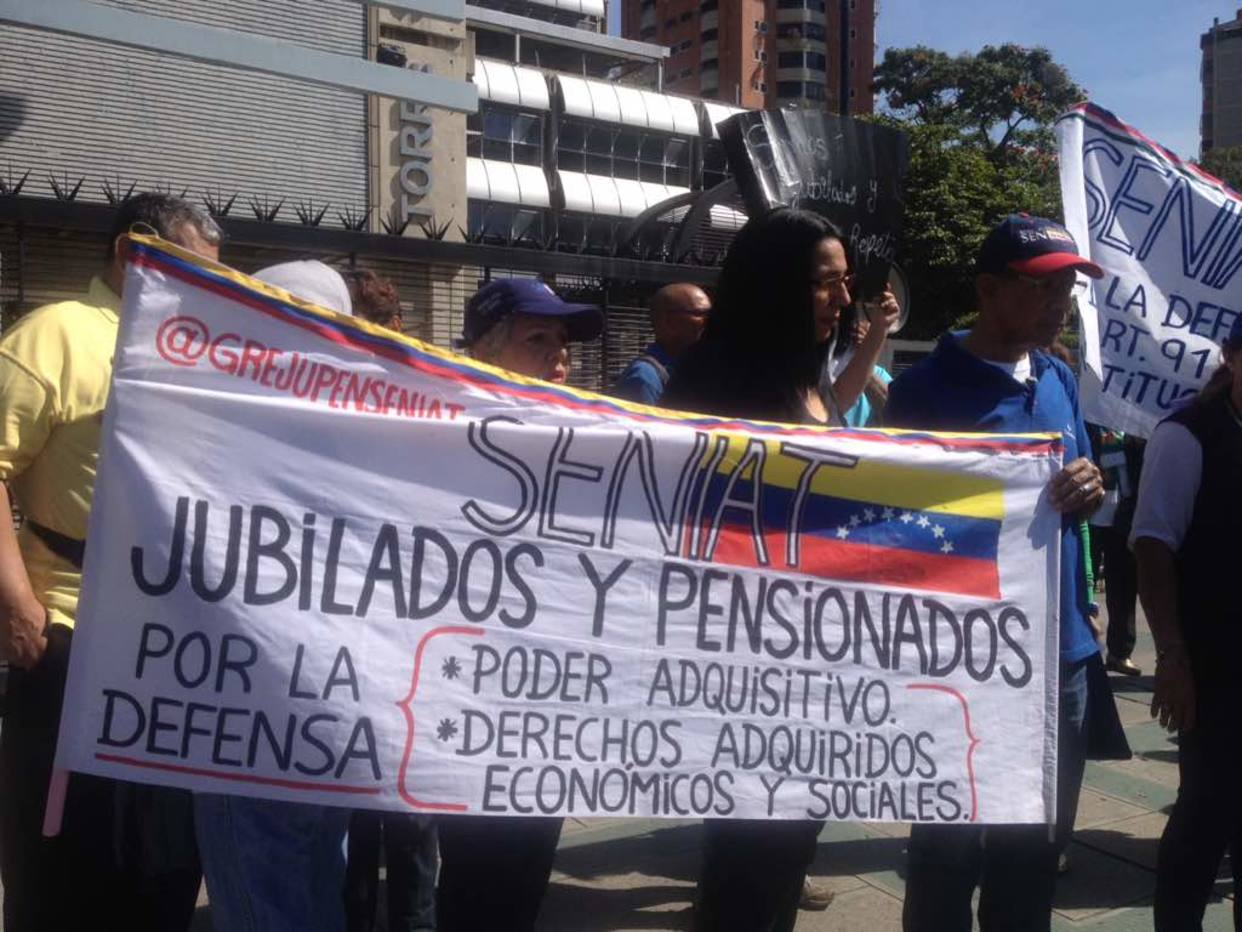
\includegraphics[width=300px]{225.jpg}%
\newline%
%
Trabajadores jubilados y activos del Seniat protestaron~este miércoles en Plaza Venezuela, Caracas, en rechazo a los bajos ingresos que reciben.%
\newline%
%
Los manifestantes aseguraron~que el dinero que perciben no les alcanza para cubrir sus necesidades, ni para comprar alimentos y medicinas.%
\newline%
%
Efectivos de la Policía Nacional Bolviariana (PNB) permanecieron~desplegados en la zona de la protesta.%
\newline%
%
\end{document}